\chapter{Data from Github}\label{github}
The biggest initial task for this thesis was the acquisition of data.
The data had to be as extensive as possible, feature a high conjunction between contributers over several repositories to verify a possible connection between those and have realistic meta data.
For these requirements two different solutions came up.


I chose Github for this purpose, as it hosts one of the biggest collection of open source projects and provides a great \ac{api} for querying Github's meta data.
A problem with this approach is that we don't have access to all important meta data, as for example the full list of members for organizations or the internal team structure of organizations.
Another problem is old email addresses, which are not related to any account anymore, because all commits made with this email address are irrefutable.
Even though some ground truth is missing, I decided to use this approach as it was still the most promising way to gather as much ground truth and real world noise as possible.


I decided to use Github as a data source, as it is not only convenient to find \acp{url} for cloning repositories, but also provides some other useful meta data, which can be used to evaluate the precision of any extracted knowledge.

Github offers some features, which are convenient to find repositories a specific user contributed to and to find other contributer which are likely related to each other.

The first feature is \emph{starring}. Every user can \emph{star} a repository to show that he likes a project.
The Github \emph{api} doesn't provide a method to get all repositories a user ever contributed to, it only allows to query the repositories owned by a user and the repositories \emph{starred} by a user.
With this feature it could be possible to get some repositories a user contributed to, even though he doesn't own these repositories, in case the user stars repositories he contributed to.

Another feature is \emph{following}. Every user can \emph{follow} another user to get informed, if they do specific things like creating new repositories or \emph{starring} repositories.
By getting the followers or following, one might catch some friends of the user.

The third feature are \emph{organizations}.
An organization is used to host projects under an account which is not necessarily led by a single natural person, but rather supports roles with different permissions and team structures.

\begin{figure}[H]
    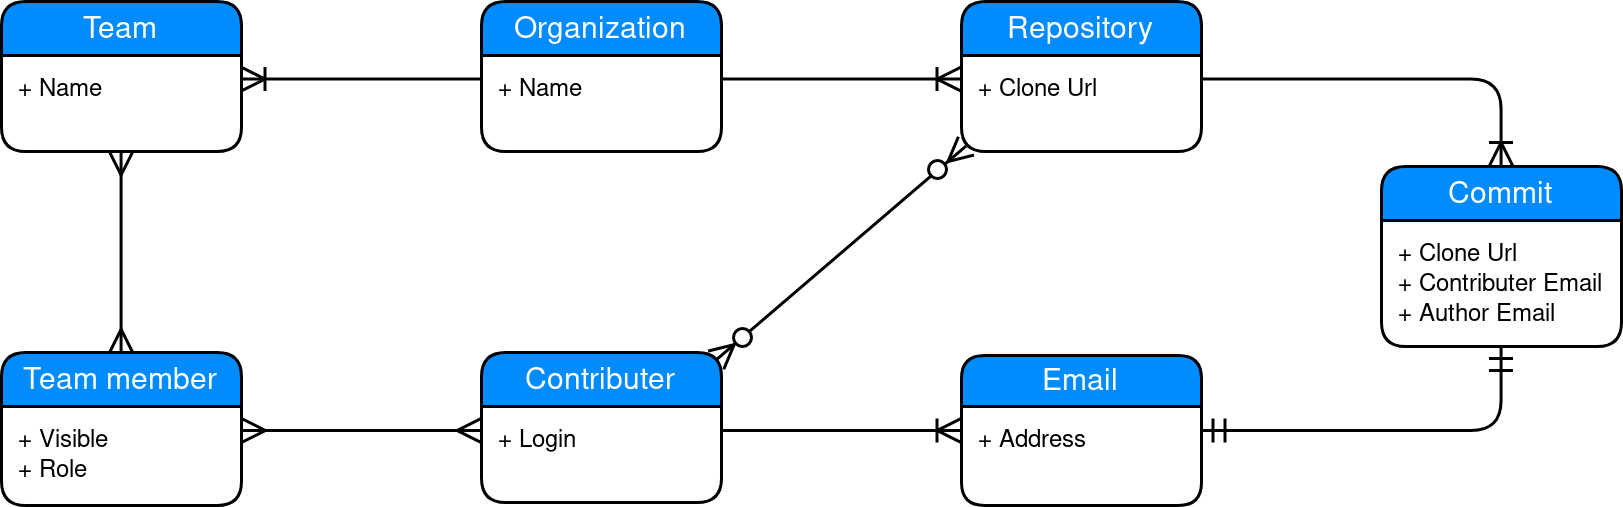
\includegraphics[scale=0.3]{./graphs/github-data-structure}
    \centering
    \caption{Simplified Github relationships.}\label{fig:github-relationship}
\end{figure}

This feature provides us with some important ground truth, but sadly a lot of information is not visible, as users have to actively opt-in, if they want to be publicly displayed as a member of an organization.
Additionally team structures can only be examined, if one is a member of the organization.
Despite not knowing all members of an organization, we still get some useful information to estimate the tendency of precision of our knowledge extraction algorithms.
